\subsubsection{\theoryC{Colored Resonance Signals at the HL- and HE-LHC}}
\contributors{Tao Han, Ian Lewis, Zhen Liu}
%\textbf{Authors: Tao Han$^{a}$, Ian Lewis$^{b}$, Zhen Liu$^{c,d}$}\\
%\textit{a) PITT-PACC, Department of Physics and Astronomy, University of Pittsburgh, PA 15260, USA\\
%b) Department of Physics and Astronomy, University of Kansas, Lawrence, KS 66045, USA\\
%c) Theoretical Physics Department, Fermi National Accelerator Laboratory, Batavia, IL, 60510\\
%d) Maryland Center for Fundamental Physics, Department of Physics, University of Maryland, College Park, MD 20742, USA
%}\\
%\texttt{than@pitt.edu, ian.lewis@ku.edu, zliu2@fnal.gov}

\newcommand\rep\mathbf

% %%%%%%%%%%%%%%%%%%%%%%%%%%%%%%%%%%%%%%%%%%%%%%
%% \subsubsection{Introduction}
\paragraph*{Introduction}
% \label{sec:intro}
% %%%%%%%%%%%%%%%%%%%%%%%%%%%%%%%%%%%%%%%%%%%%%%
With the CERN Large Hadron Collider (LHC) accumulating an unprecedented amount of data at the energy frontier, the field of high energy physics is entering an exciting new era. The high luminosity LHC (HL-LHC) will increase our knowledge of Nature and has great potential to discover new physics.  Additionally, the proposed high energy LHC (HE-LHC) at 27 TeV promises to substantially increase the chances of observation of high scale new physics.  While much of the attention for new physics discovery has centered on precision measurements of the Higgs and electroweak sectors, the LHC is a QCD machine and most initial states are composed of colored particles.  Hence, new colored dijet resonances that couple to partons will be produced with favorable rates at the HL-LHC and HE-LHC.

In a previous paper we classified the possible colored resonances at the LHC~\cite{Han:2010rf} according to their spin, electric charge, and color representation.  We now update those results for the HE-LHC.  This involves comparing the cross sections of the various resonances at the HE-LHC and HL-LHC. 

The short note is organized as follows.  In Section~\ref{par:models} we review our classifications of the different possible resonances.  Section~\ref{par:2j} we update the cross sections of dijet resonances for the HE-LHC.  Finally, in Section~\ref{par:conc} we will summarize our results and provide an outlook.

%%%%%%%%%%%%%%%%%%%%%%%%%%%%%%%%%%%%%%%%%%%%%%
%\subsubsection*{Models}
\paragraph*{Models}
\label{par:models}
%%%%%%%%%%%%%%%%%%%%%%%%%%%%%%%%%%%%%%%%%%%%%%
Most initial state at the LHC are composed of colored particles, i.e. quarks and gluons.  In this section we review the possible interactions of colored resonances and SM partons.  The resonances are classified according to their spin, electric charge, and $SU(3)_C$ color representation.  A more detailed discussion, including examples of specific realizations of the various resonances in existing literature, is given in \citeref{Han:2010rf}.  All interactions are after electroweak symmetry breaking.

Quark-quark annihilation can produce color antitriplet or sextet scalars and vectors, so-called ``diquarks''.  Please note that the diquarks under discussion here are fundamental particles and not composite.  The possible scalar diquark are denoted as  $E_{N_D},~U_{N_D}$, and $D_{N_D}$ with electric charges $4/3,2/3,-1/3$ respectively.  The subscript $N_D=3,~6$ for the $\overline{\rep3}$ and $\rep{\mathbf6}$ color representations, respectively.  Vector diquarks are represented with an additional Lorentz index $\mu$.  The interaction Lagrangian between quarks and diquarks is then
\begin{eqnarray}
\mathcal{L}_{qqD} = &K^j_{ab}& \left[ \lambda^{E}_{\alpha\beta}
E^j_{N_D}\ \overline{u^C_{\alpha a}}P_\tau u_{\beta b}
+\lambda^{U}_{\alpha\beta} U^j_{N_D}\ \overline{d^{C}_{\alpha a}}P_\tau d_{\beta b}
+\lambda^{D}_{\alpha\beta} D^j_{N_D}\ \overline{d^C_{\alpha b}}P_\tau u_{\alpha a} \right. \\
&
+&\lambda^{E'}_{\alpha\beta} E^{j\mu}_{N_D}\  \overline{u^C_{\alpha a}}\gamma_\mu P_R u_{\beta b}
+ \lambda^{U'}_{\alpha\beta}  U^{j\mu}_{N_D}\ \overline{d^C_{\alpha a}}\gamma_\mu P_R d_{\beta b}   %\nonumber\\
%&&
\left.
+\lambda^{D'}_{\alpha\beta}\ D^{j\mu}_{N_D} \overline{u^C_{\alpha a}}\gamma_\mu P_\tau d_{\beta b}
\right]
+\rm{h.c.},\nonumber
\label{eq:qq}
\end{eqnarray}
where $P_{\tau}={1\over2}(1\pm\gamma_5)$ with $\tau=R,L$ for the right- and left-chirality projection operators, $a,b$ are color indices for the $SU(3)_C$ fundamental representation, $j$ are color indices of the $N_D$ representation of $SU(3)_C$, $\alpha,\beta$ are flavor indices,  and $K^j_{ab}$ are $SU(3)_{C}$ Clebsch-Gordan (CG) coefficients.

Quarks and gluons annihilate into color triplet or antisextet fermions with $1/2$ or $3/2$ spin.  It is possible to produce a $\rep15$, but the existence of such a fermion would spoil asymptotic freedom~\cite{Chivukula:1990di}.  The spin $1/2$ ($3/2$) fermion states are denoted by $d^*_{N_D},u^*_{N_D}$ ($d^{*\mu}_{N_D},u^{*\mu}_{N_D}$) with electric charged $-1/3$ and $2/3$, respectively. The lowest order gauge invariant interactions between a gluon, quark, and heavy fermion is dimension five:  
\begin{eqnarray}
\displaystyle\mathcal{L}_{qgF} &=  \displaystyle\frac{g_{s}}{\Lambda}F^{A,\rho\sigma}
 \left[\bar u {\bar{K}_{N_D,A}} (\lambda^U_LP_L+\lambda^U_RP_R) \sigma_{\rho\sigma} u_{N_D}^{*} + \bar d {\bar{K}_{N_D,A}} (\lambda^D_LP_L+\lambda^D_RP_R) \sigma_{\rho\sigma} d_{N_D}^{*} ~~~~\right. \\
&  + \left.\bar u {\bar{K}_{N_D,A}} (\lambda^U_LP_L+\lambda^U_RP_R) \sigma_{\rho\sigma} \gamma_{\mu} u_{N_D}^{*\mu}  + \bar d {\bar{K}_{N_D,A}} (\lambda^D_LP_L+\lambda^D_RP_R) \sigma_{\rho\sigma} \gamma_{\mu} d_{N_D}^{*\mu} \right ] + \rm{h.c.}\nonumber
\label{eq:qstar}
\end{eqnarray}
where $A$ is the adjoint color index, $F^{A,\rho\sigma}$ is the gluon field strength tensor, $\sigma_{\rho\sigma}=\frac{i}{2}[\gamma_\rho,\gamma_\sigma]$, $\Lambda$ is the scale of new physics, and $K_{N_D,A}$ are $3\times N_D$ CG coefficient matrices.  

Gluon-gluon annihilation can result in many different representations, that unlike the $\rep15$ fermion do not spoil asymptotic freedom.  A complete list of the possible resonances from gluon-gluon annihilation can be found in Table 1 of \citeref{Han:2010rf}.  We will focus on the theoretically motivated color octet resonances.  Two possible resonances that can result from gluon-gluon annihilation are color octet scalars, $S_8$, and tensors, $T_8^{\mu\nu}$.  These interactions can be described in a gauge invariant way by dimension five operators:

\begin{eqnarray}
\mathcal{L}_{gg8}=g_sd^{ABC}\bigg{(}\frac{\kappa_S}{\Lambda_S} S_{8}^{A} F^B_{\mu\nu}F^{C,\mu\nu}+\frac{\kappa_{T}}{\Lambda_T}({T^{A,\mu\sigma}_8}F^{B}_{\mu\nu}{F^{C}_{\sigma}}^{~\nu}+
f {T_{8\ \rho}^{A,\rho}} \
F^{B,\mu\nu}F^C_{\mu\nu})\bigg{)},
\label{eq:tensscal}
\end{eqnarray}
where $\Lambda_{S,T}$ are the new physics scales, and the relative coupling factor $f$ is expected to be order one.  

Finally, quark-antiquark annihilation can produce color octet or singlet scalars and vectors with zero or unit charge.  The neutral vector-octet is denoted by $V^0_8$ and the  charged vector octet states $V^\pm_8$.  The interaction Lagrangian is then
\begin{eqnarray}
\mathcal{L}_{q\bar{q}V}&=&g_s\left[ {V_8}^{0,A,\mu}\ \bar{u} T^A \gamma_\mu (g^U_L P_L+g^U_{R}P_R)u+
{V_8}^{0,A,\mu}\ \bar{d} T^A \gamma_\mu (g^D_L P_L+g^D_{R}P_R)d \right .\nonumber\ \\
&&\left .+\left(V_8^{+,A,\mu}\ \bar{u} T^A \gamma_\mu (C_L V^{CKM}_LP_L+C_R V^{CKM}_R P_{R})d+\rm{h.c.}\right)\right ] ,
\label{eq:qqV}
\end{eqnarray}
where $V^{CKM}_{L,R}$ are the left- and right-handed Cabibbo-Kobayashi-Maskawa matrices, respectively.  To avoid constraints from flavor physics it is assumed that the CKM matrices align with the SM CKM matrices and that there are no tree level flavor changing neutral currents, i.e., $g^{U,D}_{L,R}$ and $C_{L,R}$ are flavor-diagonal.  To obtain the interactions with the color singlet bosons replace the representation matrices ${T^{A,a}}_b$ with the Kronecker delta ${\delta^a}_b$.  The couplings between octet and singlet scalar and light quarks is constrained to be small by minimal flavor violation~\cite{Manohar:2006ga}.  It is possible for a new scalar to have substantial couplings to the third generation quarks consistent with minimal flavor violation if it has a non-trivial representation under the SM flavor groups~\cite{Arnold:2009ay}.  We will only consider particles that couple to the light quarks and can be resonantly produced at the LHC.  Hence, we ignore scalar singlet and octet contributions to $s$-channel resonances with quark/anti-quark initial states.


\begin{table}[tb]
\caption{Summary for resonant particle names, their quantum numbers,
and possible underlying models.}
\begin{center}
\begin{tabular}{|c|c|c|c|c|c|}  \hline
 Particle Names & $J$  & $SU(3)_{C}$  & $|Q_{e}|$ & $B$ & Related models \\
 (leading coupling) &  &  &  &  &  \\ \hline
$E_{3,6}^{\mu}\ (uu)$       &0, 1& ${\rep3},\ \overline{\rep6}$ &
$4\over3$ & $ -{2\over3} $ & scalar/vector diquarks \\ \hline
$D_{3,6}^{\mu}\ (ud)$       &0, 1& ${\rep3}, \ \overline{\rep6}$ &
$1\over3$ & $ -{2\over3} $ & scalar/vector diquarks; ${\tilde d}$ \\
\hline $U_{3,6}^{\mu}\ (dd)$       &0, 1& ${\rep3},\
\overline{\rep6}$ & $2\over3$ & $ -{2\over3} $ & scalar/vector
diquarks; $\tilde u$ \\  \hline\hline
 $u^{*}_{3,6}\ (ug)$ &$1\over2$, $3\over2$& $\rep3,\ \bar{\rep6}$ & ${2\over 3}$ & $ {1\over3} $ & excited $u$;
 quixes; stringy \\ \hline
  $d^{*}_{3,6}\ (dg)$ &$1\over2$, $3\over2$& $\rep3,\ \bar{\rep6}$ & ${1\over 3}$ & $ {1\over3} $ & excited $d$;
 quixes; stringy \\  \hline\hline
 $S_{8}\ (gg)$   &0& $\rep8_{S}$ &  $0$ & $0$ & $\pi_{TC},\ \eta_{TC} $ \\ \hline
  $T_{8}\ (gg)$   &2& $\rep8_{S}$ &  $0$ & $0$ & stringy \\ \hline \hline
  $V^{0}_{8}\ (u\bar u,\ d\bar d)$      &1& $\rep8$          &  $0$   & $ 0 $  & axigluon; $g^{}_{KK},\ \rho_{TC}$; coloron \\ \hline
  $V_8^{\pm}\ (u\bar d)$  &1& $\rep8$          &  $1$   & $ 0 $  & $\rho^{\pm}_{TC}$; coloron \\ \hline
\end{tabular}
\end{center}
\label{tab:qnum}
\end{table}

In \tabb{tab:qnum} we summarize the different colored resonances discussed in this section. We list our notation for the different states along with the leading couplings to SM partons and spin, color representation, and electric charge of each state.  The subscript $S$ on $\rep8_S$ indicates that this color octet representation is the symmetric combination of two other octets, as shown in \eq{eq:tensscal}.


%%%%%%%%%%%%%%%%%%%%%%%%%%%%%%%%%%%%%%%%%%%%%%%
%\subsubsection*{Dijet Resonance Production}
\paragraph*{Dijet Resonance Production}
\label{par:2j}
%%%%%%%%%%%%%%%%%%%%%%%%%%%%%%%%%%%%%%%%%%%%%%
Since all of the resonances listed in \tabb{tab:qnum} couple to SM partons, they can decay back into SM partons.  Hence, they can be observed as dijet resonances.  We assume that the resonances decay exclusively back into (slim) dijets, i.e. not new particles or fat jets from top quarks.  If there are additional decay channels, our results can be simply rescaled by a branching ratio.
 
The cross section for resonance $R$ production via quark and/or gluon initial states at the LHC is
\begin{eqnarray}
\sigma =\mathcal{L}_{12}(\tau_0)\frac{4\pi^2}{S_H}\frac{N_D(2J_R+1)}{N_1\,N_2}\frac{\Gamma(R\rightarrow X_1 X_2)}{M_R}(1+\delta_{X_1X_2}),
\end{eqnarray}
where $X_1,X_2$ are the initial state particles, $M_R$ is the resonance mass, $S_H=14,27$~TeV is the LHC energy, and $J_R$ is the spin of the resonance.  The dimension of the color representation of the resonance and initial state particles are denoted by $N_D$ and $N_1,N_2$, respectively.  The parton luminosity is
\begin{eqnarray}
\mathcal{L}_{12}(\tau_0)=\frac{1}{1+\delta_{X_1X_2}}\int^1_{\tau_0} \frac{dx}{x}\left(f_1(x)f_2(\tau_0/x)+f_2(x)f_1(\tau_0/x)\right),
\end{eqnarray}
where $\tau_0=M_R^2/S_H$, $f_1$ is the parton distribution function (pdf) of $X_1$, and $f_2$ is the pdf of $X_2$.





\begin{figure}[tb]
\centering
%\subfigure[]{
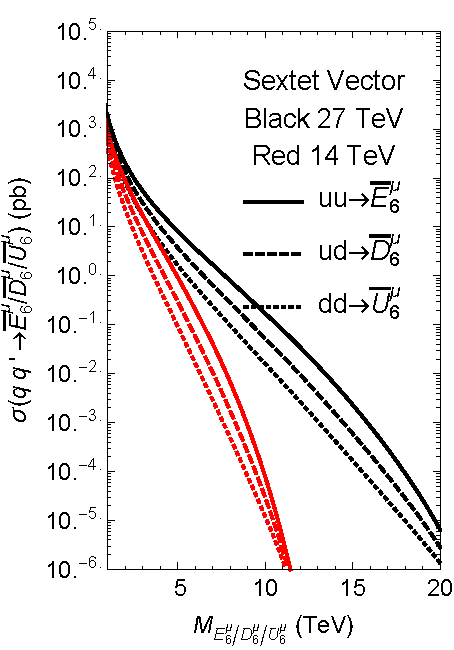
\includegraphics[width=0.24\textwidth]{\main//section7OtherSignatures/img/sextet_diquark_HE}
%}
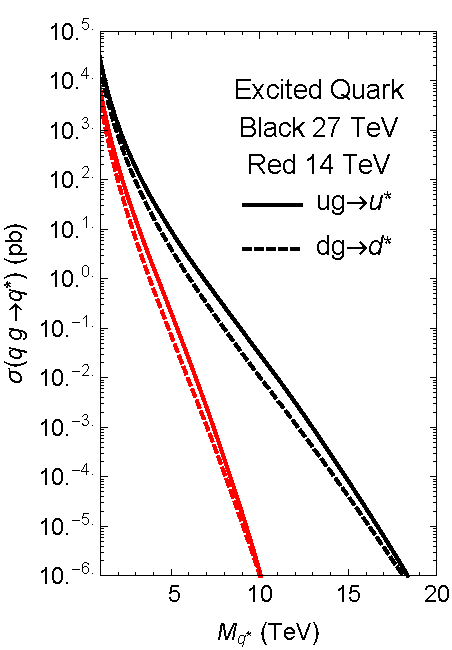
\includegraphics[width=0.24\textwidth]{\main//section7OtherSignatures/img/excited_quarks_HE}
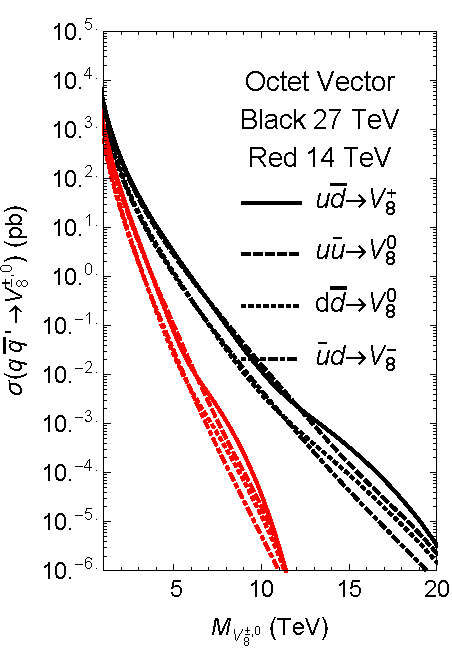
\includegraphics[width=0.24\textwidth]{\main//section7OtherSignatures/img/octet_vector_HE}
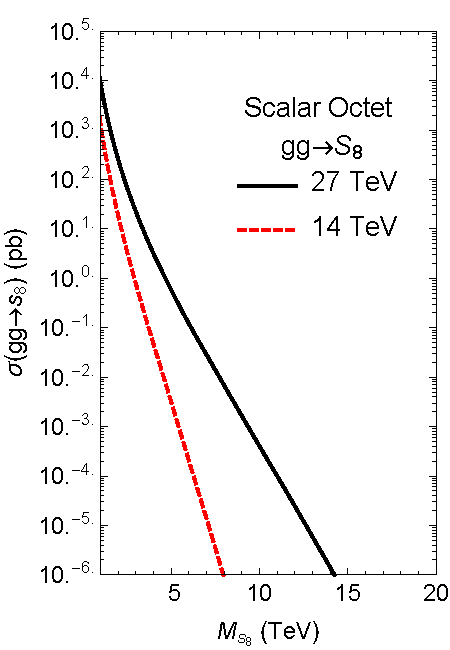
\includegraphics[width=0.24\textwidth]{\main//section7OtherSignatures/img/octet_scalar_HE}
\caption{Cross sections at HL- and HE-LHC shown in red and black curves, respectively, for (a) sextet diquarks, (b) excited quark, (c) octet vectors, and (d) $S_8$.}\label{fig:res}
\end{figure}

In \fig{fig:res} we show the cross sections of (a) sextet diquarks, (b) excited quarks, (c) octet vectors, and (d) $S_8$ for both the (red) HL- and (black) HE-LHC.  These cross sections are calculated using the NNPDF~\cite{Ball:2014uwa} pdf set, the coupling constants $\lambda^{E,U,D}$,$\kappa_S$ are set to one, and the new physics scales $\Lambda=\Lambda_S=M_R$.    The sextet scalar cross sections are the largest for large resonance mass due to an enhancement from having two valence quarks in the initial state.  Somewhat surprisingly, despite the LHC having a reputation as having a large gluon pdf, at very high masses the vector octets produced from quark/anti-quark initial states have larger cross sections than resonances from gluon initial states.  This is because the gluon pdf drops precipitously at high momentum fraction.  In fact, at the highest resonance masses, $S_8$ produced from gluon fusion has the lowest cross sections.  Although the precise value of these rates depend on the choices of couplings and new physics scale, the gluon pdf suppression is clearly seen by how quickly the excited quark and $S_8$ cross sections decrease at high resonance masses as compared to the vector octets.

As can be clearly seen, the cross sections greatly increase at the HE-LHC.  For a resonance mass around $10-11$ TeV, we might expect $\mathcal{O}(1)$ events at the HL-LHC with 3 ab$^{-1}$ of data for diquarks, excited quarks, and vector octets. For these resonances and resonance mass, at the HE-LHC with 3 ab$^{-1}$ of data we may expect $\mathcal{O}(1,000-100,000)$ events.  For $S_8$, for a resonance mass of 8 TeV for 3 ab$^{-1}$ we expect $\mathcal{O}(1)$ events at the HL-HLC and $\mathcal{O}(10,000)$ events at the HE-LHC.   This is a factor of $\mathcal{O}(1,000-100,000)$ increase in the cross sections at the HE-LHC.

Additionally, at the HE-LHC, the mass reach is considerably extended.  The baseline for the HE-LHC is 15 ab$^{-1}$ by its end run.  For 15 ab$^{-1}$ we expect $\mathcal{O}(10)$ events for 21 TeV diquarks ($E_6^u$), 19 TeV excited quark ($u^*$), 21 TeV octet vectors ($V_8^+$), and 15 TeV octet scalar $S_8$.  Comparing this to the masses for which we expect $\mathcal{O}(10)$ events by the end of the HL-LHC, we see that we may expect the mass reach of the HE-LHC to be twice the HL-LHC.

%%%%%%%%%%%%%%%%%%%%%%%%%%%%%%%%%%%%%%%%%%%%%%
%\subsubsection*{Conclusions}
\paragraph*{Conclusions}
\label{par:conc}

The LHC is a QCD machine and colored resonances that couple to partons are expected to be produced at favorable rates.  Since these resonances couple to partons, they can be observed as dijet resonances. We have updated our previous analysis of these resonances~\cite{Han:2010rf} for the HL- and HE-LHC.  We have reviewed the classification of these resonances according to spin, electric charge, and color representation as well as their couplings to Standard Model partons.  The cross sections of sextet diquarks, excited quarks, vector octets, and a scalar octet coupling to gluons were calculated.  Using the benchmark scenarios of 3 ab$^{-1}$ at 14 TeV for the HL-LHC and 15 ab$^{-1}$ at 27 TeV for the HE-LHC, we find that that the HE-LHC is sensitive to resonance masses up to a factor of two larger than the HL-LHC.
%%%%%%%%%%%%%%%%%%%%%%%%%%%%%%%%%%%%%%%%%%%%%%

%\bibliography{ref}
%\bibliographystyle{JHEP}
%\bibliography{\main//section7OtherSignatures/bib/coloreddijet}
